% Déclaration du type de document (report, book, paper, etc...)
\documentclass[a4paper]{paper} 
 
% Package pour avoir Latex en français
\usepackage[utf8]{inputenc}
\usepackage[T1]{fontenc}
 
% Quelques packages utiles
\usepackage{listings} % Pour afficher des listings de programmes
\usepackage{graphicx} % Pour afficher des figures
\usepackage{amsthm}   % Pour créer des théorèmes et des définitions
\usepackage{amsmath}
\usepackage{microtype} % Optical margins FTW
\usepackage{url}
\usepackage{booktabs} % Allows the use of \toprule, \midrule and \bottomrule in tables for horizontal lines
\usepackage{siunitx}
\usepackage{floatrow}
\usepackage{caption}
\usepackage{subcaption}
\usepackage{mhchem}
\usepackage[acronym,smallcaps]{glossaries}


% Début du document
\begin{document}
\begin{titlepage}

\newcommand{\HRule}{\rule{\linewidth}{0.5mm}} % Defines a new command for the horizontal lines, change thickness here

\center % Center everything on the page 
%----------------------------------------------------------------------------------------
%	HEADING 
%----------------------------------------------------------------------------------------
\textsc{\LARGE Club Vaudois de Robotique Autonome}\\[1.5cm] 

%----------------------------------------------------------------------------------------
%	TITLE 
%----------------------------------------------------------------------------------------
\HRule \\[0.4cm]
{ \huge \bfseries Eurobot 2014 : Pilot Study}\\[0.4cm] % Title of your document
\HRule \\[1.5cm]
 
%----------------------------------------------------------------------------------------
% LOGO EPFL
%----------------------------------------------------------------------------------------
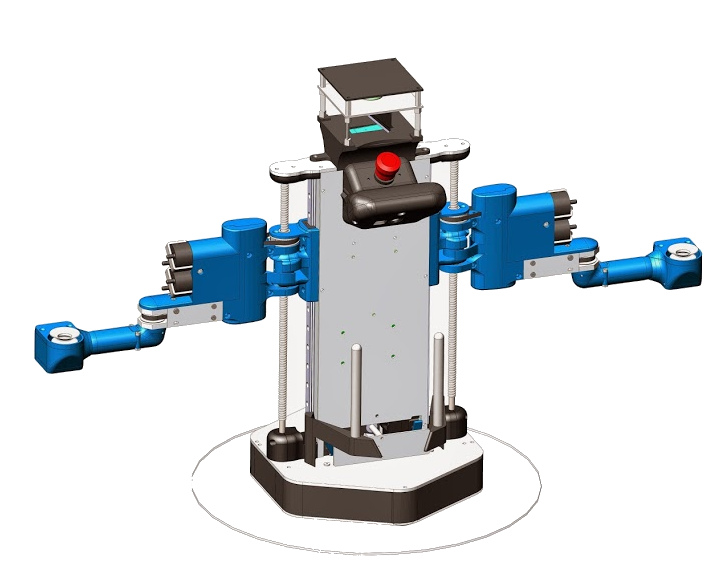
\includegraphics[width=\textwidth]{images/Debra_IV_1}\\[2cm] 

%----------------------------------------------------------------------------------------
%	AUTHORS 
%----------------------------------------------------------------------------------------

\vfill % Fill the rest of the page with whitespace

{\large \today}
\end{titlepage}




\section{General information}
\begin{itemize}
    \item This project study can be published before the contest.
    \item Team name : CVRA (Club Vaudois de Robotique Autonome).
    \item Team location : Renens, Switzerland.
    \item Budget : About 3000 \textsc{chf}, plus sponsors.
\end{itemize}

\section{Robots}
This year the club will engage two robots which are evolutions of previous years' designs.
The first one will have two arms, a differential drive and has code name ``Debra 4''.
The second one will have an holonomic base, and is nicknamed ``Nastya 2''.

\subsection{Debra 4}
\begin{figure}[h]
    \begin{center}
        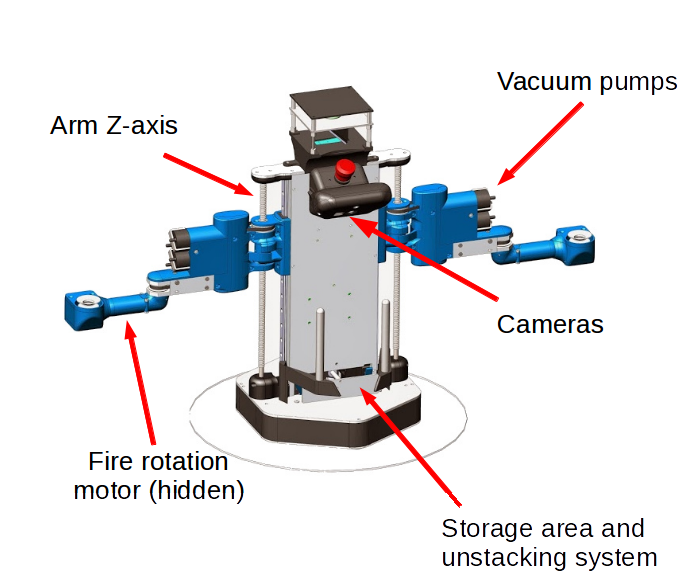
\includegraphics[width=0.6\textwidth]{images/debra_explained}
        \caption{Debra 4 robot.
            Height : \SI{350}{\milli\meter}.
            Perimeter : \SI{695}{\milli\meter}.
        }
        \label{fig:balise}
    \end{center}
\end{figure}
Debra 4 is our biggest robot, dedicated to rotating the fire on the correct side, although fruits may be implemented if time allows it.
At the beginning of the game, it will quickly go to the fires' positions and take them with its arms (using vacuum).
It can then find the orientation of the fire using fixed color sensors and store them in front of the robot.
For unloading the fire, Debra can either unstack them using its arms or it can push them out from the bottom of the stack using a small lever.

\paragraph{Motors}
Debra 4 uses two Faulhaber 2232-012-SR motors with a 20:1 reduction, rated at \SI{8.7}{\watt} at \SI{12}{\volt}, overvolted at \SI{14.8}{\volt}.
Those motors allows us to use our max acceleration (wheel slippage) to \SI{0.8}{\meter\per\second}.
All the motors in the robots are driven using custom power electronics.

\paragraph{Positioning}
Debra 4 will use a standard, encoder-based odometry to find its position on the table.
We will also use an inertial measurement unit to have an additional source of information.
These two techniques will be merged using a Kalman filter.

\paragraph{Opponent detection}
We have planned to build an optical absolute positioning beacon system, but it may not be ready for the contest due to the complexity of the project.
If we cannot make it in time, we will fall back on last year's beacon system (fig. \ref{fig:balise}).
The relative simplicity of this second design makes it very reliable and easy to implement, which guarantees that it will be ready for the Belgium and Switzerland contests.

\paragraph{Power supply}
The robot is powered by a single \SI{14.8}{\volt} lithium-polymer battery, which gives us a run time of at least \SI{40}{\minute}.

\begin{figure}[h]
    \begin{center}
        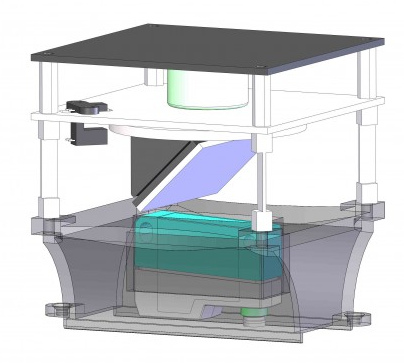
\includegraphics[width=0.6\textwidth]{images/Balise}
        \caption{Fallback beacon system.
            A reflex-type industrial sensor is mounted in the base (blue).
            It emits a LED beam (not laser), which is reflected on the rotating mirror (purple).
            A reflector is placed on the opponent robot, which allows for reliable detection.
            An index sensor (upper left, black) allows the robot to know the relative angle to opponent.
        }
        \label{fig:balise}
    \end{center}
\end{figure}



\paragraph{Sensors}
In addition to the encoders and the beacon system, Debra has a few sensors to find the current orientation (color) of the fires.
The two main sensors for this application are two Sick color sensors, mounted on the side of the robot.
To measure a fire's color, the robot must take it with one arm and approach it near the sensor.
We also have a range camera to find the fire's location which is combined to a color camera for decision making.

\paragraph{Computing}
Both of our robots have two processing unit :
\begin{itemize}
    \item An x86-based embedded PC running Linux is used for computer vision, path planning and state synchronization with Nastya (WLAN link).
    \item An FPGA board with an Altera Nios 2 softcore processor is used for real time operations, such as motor control.
        We run UC/OS-II on this board, an industrial and proven RTOS, free for academic and hobby use.
\end{itemize}

The two boards communicate via TCP/IP over serial, which make communication testing and debugging very easy thanks to tool like Wireshark.

\subsection{Nastya 2}
\begin{figure}[h]
    \begin{center}
        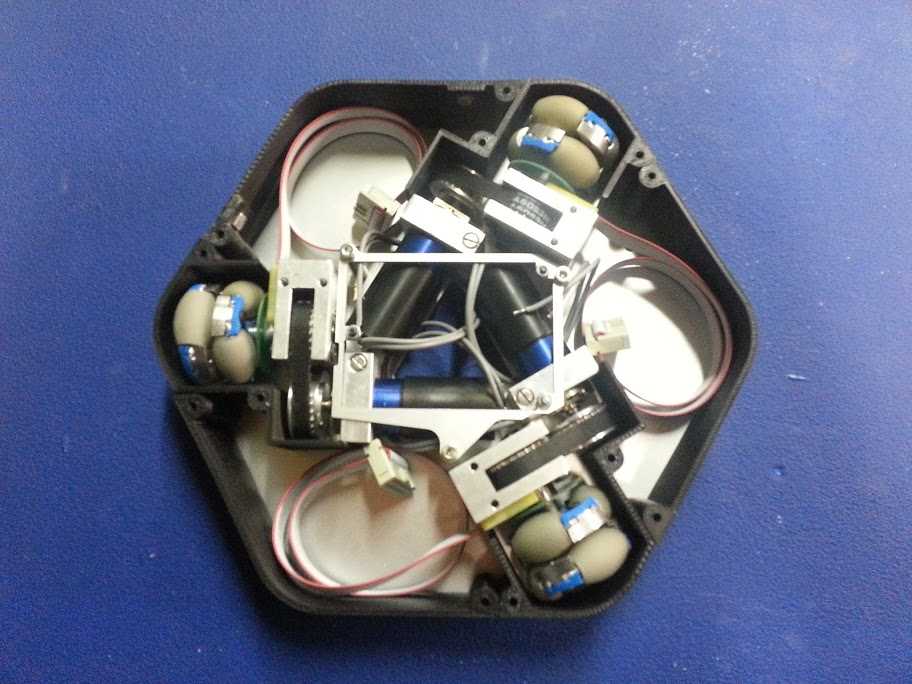
\includegraphics[width=0.6\textwidth]{images/Nastya_I}
        \caption{
            Nastya original version (2013).
            The second version will be mostly the same with a scale up to reach the new perimeter of \SI{695}{\milli\meter}.
            The CAD of Nastya 2 is not complete yet.
        }
        \label{fig:balise}
    \end{center}
\end{figure}
Nastya 2 is our secondary robot, responsible for the spears, frescos and mammoths capture.
As it has shares many design decision with Debra, only differences will be presented.

\paragraph{Motors}
Nastya uses 3 motors instead of only 2 because of its holonomic drive.
The holonomic wheels are custom made to reduce play and allow for better precision.


\paragraph{Sensors}
We \emph{may} have sensors on Nastya 2.
Have not decided yet.
Sensors are nice.
I like sensors.



\section{Team members}
\begin{itemize}
    \item Antoine Albertelli, 21:  Lead programmer, Debra 4.
    \item Florian Reinhard, XX:  Lead programmer, Nastya 2.
    \item Patrick Spieler, XX:  Inter-board communication.
    \item Pius von Däniken, XX:  Motion planning.
    \item Romain Bersier, 29:  Mechanical engineer, Debra 4.
    \item Boris Pillionnel, 23:  Mechanical engineer, Nastya 2.
    \item Patrick Eugster, 29:  Electrical engineer.
    \item Mathieu Rouvinez, XX:  Machining and mathematical wizardry.
    \item Guillaume Doe, XX: Mechanical engineer.
    \item Jessica Doe: Electrical engineer:
    \item Thierry Prêtre, 21:  Sponsoring and public relationships.
\end{itemize}

\clearpage


\section{Sponsors}
\begin{figure}[h!]
    \centering
    \begin{subfigure}[h]{0.15\textheight}
        
\includegraphics[width=\textwidth]{images/sponsors/altera}
    \end{subfigure}%
    \hspace{1cm}
    \begin{subfigure}[h]{0.15\textheight}
        
\includegraphics[width=\textwidth]{images/sponsors/arrow}
    \end{subfigure}
    \vspace{0.4cm}


\vspace{0.4cm}


    \begin{subfigure}[h]{0.15\textheight}
        
\includegraphics[width=\textwidth]{images/sponsors/bossard}
    \end{subfigure}%
    \hspace{1cm}
    \begin{subfigure}[h]{0.15\textheight}
        
\includegraphics[width=\textwidth]{images/sponsors/claudePiguet}
    \end{subfigure}
\vspace{0.4cm}


    \begin{subfigure}[h]{0.15\textheight}
        
\includegraphics[width=\textwidth]{images/sponsors/faulhaber}
    \end{subfigure}%
    \hspace{1cm}
    \begin{subfigure}[h]{0.15\textheight}
        
\includegraphics[width=\textwidth]{images/sponsors/festo}
    \end{subfigure}
\vspace{0.4cm}


    \begin{subfigure}[h]{0.15\textheight}
        
\includegraphics[width=\textwidth]{images/sponsors/gardnerDenverThomas}
    \end{subfigure}%
    \hspace{1cm}
    \begin{subfigure}[h] {0.15\textheight}
        
\includegraphics[width=\textwidth]{images/sponsors/jauslin}
    \end{subfigure}
\vspace{0.4cm}


    \begin{subfigure}[h]{0.15\textheight}
        
\includegraphics[width=\textwidth]{images/sponsors/omron}
    \end{subfigure}%
    \hspace{1cm}
    \begin{subfigure}[h]{0.15\textheight}
        
\includegraphics[width=\textwidth]{images/sponsors/phoenixContact}
    \end{subfigure}
\vspace{0.4cm}


    \begin{subfigure}[h]{0.15\textheight}

        
\includegraphics[width=\textwidth]{images/sponsors/skf}
    \end{subfigure}%
    \hspace{1cm}
    \begin{subfigure}[h]{0.15\textheight}
        
\includegraphics[width=\textwidth]{images/sponsors/posic}
    \end{subfigure}
\vspace{0.4cm}


    \begin{subfigure}[h]{0.15\textheight}
        
\includegraphics[width=\textwidth]{images/sponsors/renens}
    \end{subfigure}%
    \hspace{1cm}
    \begin{subfigure}[h]{0.15\textheight}
        
\includegraphics[width=\textwidth]{images/sponsors/sick}
    \end{subfigure}
\vspace{0.4cm}


    \begin{subfigure}[h]{0.15\textheight}
        
\includegraphics[width=\textwidth]{images/sponsors/pmd}
    \end{subfigure}%
    \hspace{1cm}
    \begin{subfigure}[h]{0.15\textheight}
        
\includegraphics[width=\textwidth]{images/sponsors/SwissCNCTechnologies}
    \end{subfigure}
\vspace{0.4cm}


    \begin{subfigure}[h]{0.15\textheight}
        
\includegraphics[width=\textwidth]{images/sponsors/SwissMeo}
    \end{subfigure}%
    \hspace{1cm}
    \begin{subfigure}[h]{0.15\textheight}
        
\includegraphics[width=\textwidth]{images/sponsors/techniquesLaser}
    \end{subfigure}
\vspace{0.4cm}


\end{figure}





\end{document}
